\let\negmedspace\undefined
\let\negthickspace\undefined
\documentclass[journal,12pt,onecolumn]{IEEEtran}
\usepackage{cite}
\usepackage{amsmath,amssymb,amsfonts,amsthm}
\usepackage{algorithmic}
\usepackage{graphicx}
\graphicspath{{./figs/}}
\usepackage{textcomp}
\usepackage{xcolor}
\usepackage{txfonts}
\usepackage{listings}
\usepackage{enumitem}
\usepackage{mathtools}
\usepackage{gensymb}
\usepackage{comment}
\usepackage{caption}
\usepackage[breaklinks=true]{hyperref}
\usepackage{tkz-euclide} 
\usepackage{listings}
\usepackage{gvv}                                        
%\def\inputGnumericTable{}                                 
\usepackage[latin1]{inputenc}     
\usepackage{xparse}
\usepackage{color}                                            
\usepackage{array}                                            
\usepackage{longtable}                                       
\usepackage{calc}                                             
\usepackage{multirow}
\usepackage{multicol}
\usepackage{hhline}                                           
\usepackage{ifthen}                                           
\usepackage{lscape}
\usepackage{tabularx}
\usepackage{array}
\usepackage{float}
\newtheorem{theorem}{Theorem}[section]
\newtheorem{problem}{Problem}
\newtheorem{proposition}{Proposition}[section]
\newtheorem{lemma}{Lemma}[section]
\newtheorem{corollary}[theorem]{Corollary}
\newtheorem{example}{Example}[section]
\newtheorem{definition}[problem]{Definition}
\newcommand{\BEQA}{\begin{eqnarray}}
\newcommand{\EEQA}{\end{eqnarray}}
\newcommand{\define}{\stackrel{\triangle}{=}}
\theoremstyle{remark}
\newtheorem{rem}{Remark}



\title{\LARGE \textbf{AE - 2021}}
\author{\Large EE25BTECH11048 - Revanth Siva Kumar.D}
\date{}

\begin{document}

\maketitle
\begin{flushleft}
\begin{center}
\large\textbf{General Aptitude (GA)}
\end{center}

\textbf{ Q.1 -- Q.5 Multiple Choice Question (MCQ), carry ONE mark each (for each wrong answer: $-\dfrac{1}{3}$).}

\begin{enumerate}
\item 
(i) Arun and Aparna are here. \\
(ii) Arun and Aparna is here. \\
(iii) Arun's families is here. \\
(iv) Arun's family is here. \\

Which of the above sentences are grammatically CORRECT?

\hfill (GATE AE 2021)

\begin{enumerate}
\begin{multicols}{2}
\item (i) and (ii)
\item (i) and (iv)
\item (ii) and (iv)
\item (iii) and (iv)
\end{multicols}
\end{enumerate}


\item 
The mirror image of the above text about the x-axis is \begin{figure}[H]
    \centering
    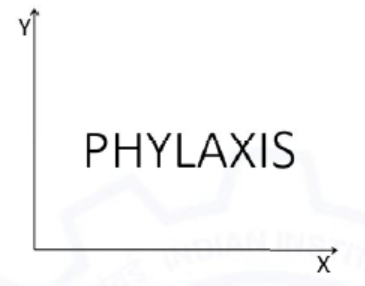
\includegraphics[width=0.5\columnwidth]{figs/Q2.png}
    \caption{}
    \label{fig:placeholder}
\end{figure}


\hfill (GATE AE 2021)

\begin{enumerate}
\begin{multicols}{2}
\item 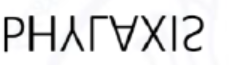
\includegraphics[width=0.5\columnwidth]{figs/1.png}
\item 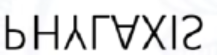
\includegraphics[width=0.5\columnwidth]{figs/2.png}
\item 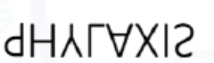
\includegraphics[width=0.5\columnwidth]{figs/3.png}
\item 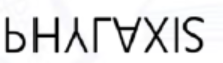
\includegraphics[width=0.5\columnwidth]{figs/4.png}
\end{multicols}
\end{enumerate}
\item 
Two identical cube shaped dice each with faces numbered $1$ to $6$ are rolled simultaneously. The probability that an even number is rolled out on each dice is:

\hfill (GATE AE 2021)
\begin{enumerate}
\begin{multicols}{2}
\item $\dfrac{1}{36}$
\item $\dfrac{1}{12}$
\item $\dfrac{1}{8}$
\item $\dfrac{1}{4}$
\end{multicols}
\end{enumerate}

\item 
$\oplus$ and $\odot$ are two operators on numbers $p$ and $q$ such that \\
$p \odot q = p - q, \quad p \oplus q = p \times q$ \\

Then, $(9 \odot (6 \oplus 7)) \odot (7 \oplus (6 \odot 5)) =$ 
\hfill (GATE AE 2021)
\begin{enumerate}
\begin{multicols}{2}
\item 40
\item -26
\item -33
\item -40
\end{multicols}
\end{enumerate}


\item 
Four persons P, Q, R and S are to be seated in a row. R should not be seated at the second position from the left end of the row. The number of distinct seating arrangements possible is:
\hfill (GATE AE 2021)
\begin{enumerate}
\begin{multicols}{2}
\item 6
\item 9
\item 18
\item 24
\end{multicols}
\end{enumerate}
\textbf{Q.6 -- Q.10 Multiple Choice Question (MCQ), carry TWO marks each (for each wrong answer: $-\dfrac{2}{3}$).}

\item 
On a planar field, you travelled $3$ units East from a point O. Next you travelled $4$ units South to arrive at point P. Then you travelled from P in the North-East direction such that you arrive at a point that is $6$ units East of point O. Next, you travelled in the North-West direction, so that you arrive at point Q that is $8$ units North of point P. \\

The distance of point Q to point O, in the same units, should be \underline{\hspace{2cm}}
\hfill (GATE AE 2021)
\begin{enumerate}
\begin{multicols}{2}
\item 3
\item 4
\item 5
\item 6
\end{multicols}
\end{enumerate}

\item 
The author said, ``Musicians rehearse before their concerts. Actors rehearse their roles before the opening of a new play. On the other hand, I find it strange that many public speakers think they can just walk on to the stage and start speaking. In my opinion, it is no less important for public speakers to rehearse their talks.'' \\

Based on the above passage, which one of the following is TRUE?
\hfill (GATE AE 2021)
\begin{enumerate}
\begin{multicols}{2}
\item The author is of the opinion that rehearsing is important for musicians, actors and public speakers.
\item The author is of the opinion that rehearsing is less important for public speakers than for musicians and actors.
\item The author is of the opinion that rehearsing is more important only for musicians than public speakers.
\item The author is of the opinion that rehearsal is more important for actors than musicians.
\end{multicols}
\end{enumerate}

\item 
1.\textbf{Some football players play cricket.} \\
2.\textbf{All cricket players play hockey.} \\

Among the options given below, the statement that logically follows from the two statements 1 and 2 above, is:
\hfill (GATE AE 2021)
\begin{enumerate}
\begin{multicols}{2}
\item No football player plays hockey.
\item Some football players play hockey.
\item All football players play hockey.
\item All hockey players play football.
\end{multicols}
\end{enumerate}

\item 
\begin{figure}
    \centering
    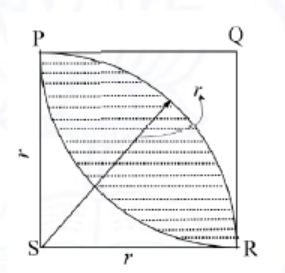
\includegraphics[width=0.3\columnwidth]{figs/q9.png}
    \caption{}
    \label{fig:placeholder}
\end{figure}

In the figure shown above, PQRS is a square. The shaded portion is formed by the intersection of sectors of circles with radius equal to the side of the square and centers at S and Q. \\

The probability that any point picked randomly within the square falls in the shaded area is \underline{\hspace{2cm}}
\hfill (GATE AE 2021)
\begin{enumerate}
\begin{multicols}{2}
\item $4 - \dfrac{\pi}{2}$
\item $\dfrac{1}{2}$
\item $\dfrac{\pi}{2} - 1$
\item $\dfrac{\pi}{4}$
\end{multicols}
\end{enumerate}
\item 
In an equilateral triangle PQR, side PQ is divided into four equal parts, side QR is divided into six equal parts and side PR is divided into eight equal parts. The length of each subdivided part in cm is an integer. \\

The minimum area of the triangle PQR possible, in cm$^2$, is \underline{\hspace{2cm}}

\hfill (GATE AE 2021)

\begin{enumerate}
\begin{multicols}{2}
\item $18$
\item $24$
\item $48\sqrt{3}$
\item $144\sqrt{3}$
\end{multicols}
\end{enumerate}
\end{enumerate}

\begin{center}
\textbf{Aerospace Engineering (AE)}
\end{center}

\textbf{ Q.1 -- Q.13 Multiple Choice Question (MCQ), carry ONE mark each (for each wrong answer: $-\dfrac{1}{3}$).}

\begin{enumerate}
\item Consider the differential equation
\begin{align*}
\dfrac{d^2 y}{dx^2} + 8\dfrac{dy}{dx} + 16y &= 0
\end{align*}
and the boundary conditions
\begin{align*}
y(0) &= 1, \quad \dfrac{dy}{dx}(0) = 0
\end{align*}
The solution to this equation is

\hfill (GATE AE 2021)

\begin{enumerate}
\begin{multicols}{2}
\item $y = (1+2x)e^{-4x}$
\item $y = (1-4x)e^{-4x}$
\item $y = (1+8x)e^{-4x}$
\item $y = (1+4x)e^{-4x}$
\end{multicols}
\end{enumerate}


\item 
$u(x,y)$ is governed by the following equation
\begin{align*}
\dfrac{\partial^2 u}{\partial x^2} - 4\dfrac{\partial^2 u}{\partial x \partial y} + 6\dfrac{\partial^2 u}{\partial y^2} &= x + 2y
\end{align*}
The nature of this equation is

\hfill (GATE AE 2021)

\begin{enumerate}
\begin{multicols}{2}
\item linear
\item elliptic
\item hyperbolic
\item parabolic
\end{multicols}
\end{enumerate}

\item 
Consider the velocity field 
\begin{align*}
\vec{V} &= (2x+3y)\,\hat{i} + (3x+2y)\,\hat{j}
\end{align*}
The field $\vec{V}$ is

\hfill (GATE AE 2021)

\begin{enumerate}
\begin{multicols}{2}
\item divergence-free and curl-free
\item curl-free but not divergence-free
\item divergence-free but not curl-free
\item neither divergence-free nor curl-free
\end{multicols}
\end{enumerate}

\item 
The figure shows schematics of wave patterns at the exit of nozzles A and B operating at different pressure ratios. 
\begin{figure}[H]
    \centering
    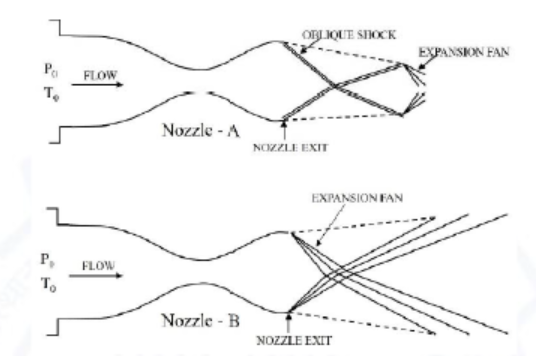
\includegraphics[width=0.5\columnwidth]{figs/q1 4.png}
    \caption{}
    \label{fig:placeholder}
\end{figure}
Nozzles A and B, respectively, are said to be operating in:

\hfill (GATE AE 2021)

\begin{enumerate}
\item over-expanded mode and under-expanded mode
\item under-expanded mode and perfectly expanded mode
\item perfectly expanded mode and under-expanded mode
\item under-expanded mode and over-expanded mode

\end{enumerate}
\item 
The combustion process in a turbo-shaft engine during ideal operation is:

\hfill (GATE AE 2021)

\begin{enumerate}
\begin{multicols}{2}
\item isentropic
\item isobaric
\item isochoric
\item isothermal
\end{multicols}
\end{enumerate}

\item 
How does the specific thrust of a turbojet engine change for a given flight speed with increase in flight altitude?

\hfill (GATE AE 2021)

\begin{enumerate}
\begin{multicols}{2}
\item Increases monotonically
\item Decreases monotonically
\item Remains constant
\item First increases and then decreases
\end{multicols}
\end{enumerate}
\item 
How does the propulsion efficiency of a turbofan engine, operating at a given Mach number and a given altitude, change with increase in compressor pressure ratio?

\hfill (GATE AE 2021)

\begin{enumerate}
\item Remains constant
\item Increases monotonically
\item Decreases monotonically
\item First decreases and then increases
\end{enumerate}

\item 
A solid propellant rocket producing thrust for a duration is fired. The specific impulse is given. 
\begin{align*}
T &= 25\,\text{MN}, \quad t = 150\,\text{s}, \quad I_{sp} = 2980\,\text{N s/kg}
\end{align*}
How much propellant is burned during the rocket operation?

\hfill (GATE AE 2021)

\begin{enumerate}
\item 8390 kg
\item 82300 kg
\item $1.26 \times 10^{6}$ kg
\item $11.2 \times 10^{6}$ kg
\end{enumerate}
\item 
The shape of a supersonic diffuser that slows down a supersonic flow to subsonic flow is

\hfill (GATE AE 2021)

\begin{enumerate}
\begin{multicols}{2}
\item converging
\item diverging
\item diverging--converging
\item converging--diverging
\end{multicols}
\end{enumerate}

\item 
Uniaxial tension test (see the figure) is conducted on two different samples prepared with homogeneous, isotropic materials. One of the materials is brittle, whereas the other is ductile.
\begin{figure}[H]
    \centering
    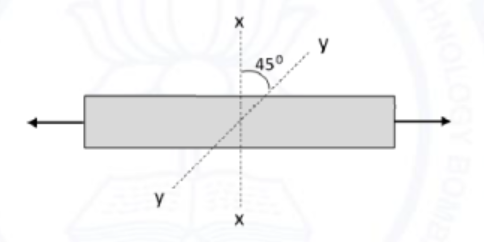
\includegraphics[width=0.5\columnwidth]{figs/qq.png}
    \caption{}
    \label{fig:placeholder}
\end{figure}
Assuming that there is no stress concentration at loading points, the failure would initiate:

\hfill (GATE AE 2021)

\begin{enumerate}
\item along x--x in both materials
\item along x--x in brittle material and along y--y in ductile material
\item along y--y in brittle material and along x--x in ductile material
\item along y--y in both materials
\end{enumerate}
\item 
For the state of stress as shown in the figure, what is the orientation of the plane with maximum shear stress with respect to the x-axis?
\begin{figure}[H]
    \centering
    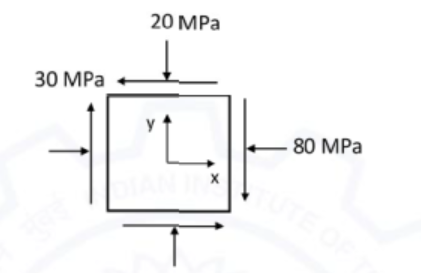
\includegraphics[width=0.5\columnwidth]{figs/11.png}
    \caption{}
    \label{fig:placeholder}
\end{figure}
\hfill (GATE AE 2021)

\begin{enumerate}
\begin{multicols}{2}
\item $45\degree$
\item $-45\degree$
\item $22.5\degree$
\item $-22.5\degree$
\end{multicols}
\end{enumerate}

\item 
Let $V_{\text{TAS}}$ be the true airspeed of an aircraft flying at a certain altitude where the density of air is $\rho$, and $V_{\text{EAS}}$ be the equivalent airspeed. If $\rho_0$ is the density of air at sea level, what is the ratio
\begin{align*}
\dfrac{V_{\text{TAS}}}{V_{\text{EAS}}}\; ?
\end{align*}

\hfill (GATE AE 2021)

\begin{enumerate}
\begin{multicols}{2}
\item $\dfrac{\rho}{\rho_0}$
\item $\dfrac{\rho_0}{\rho}$
\item $\sqrt{\dfrac{\rho_0}{\rho}}$
\item $\sqrt{\dfrac{\rho}{\rho_0}}$
\end{multicols}
\end{enumerate}
\item $C_m - \alpha$ variation for a certain aircraft is shown in the figure. Which one of the following statements is true for this aircraft?

\begin{figure}[H]
    \centering
    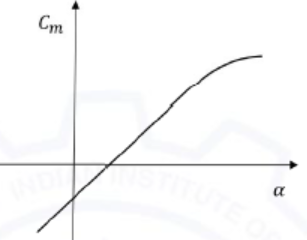
\includegraphics[width=0.5\columnwidth]{figs/12.png}
    \caption{}
    \label{fig:placeholder}
\end{figure}


\hfill (GATE AE 2021)

\begin{enumerate}
\item The aircraft can trim at a positive $\alpha$ and it is stable.
\item The aircraft can trim at a positive $\alpha$, but it is unstable.
\item The aircraft can trim at a negative $\alpha$ and it is stable.
\item The aircraft can trim at a negative $\alpha$, but it is unstable.
\end{enumerate}
\textbf{Q.14 -- Q.16 Multiple Select Question (MSQ), carry ONE mark each (no negative marks).}

\item 
Which of the following statement(s) is/are true across an oblique shock (in adiabatic conditions) over a wedge shown below?
\begin{figure}[H]
    \centering
    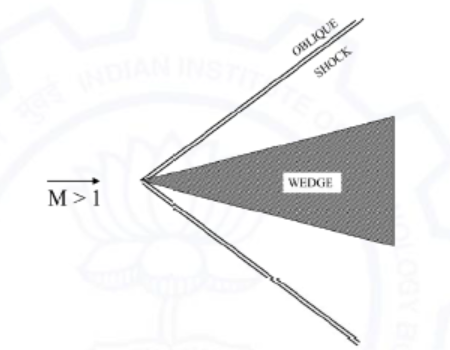
\includegraphics[width=0.5\columnwidth]{figs/13.png}
    \caption{}
    \label{fig:placeholder}
\end{figure}
\hfill (GATE AE 2021)

\begin{enumerate}
\item Total pressure decreases
\item Mach number based on velocity tangential to the shock decreases
\item Total temperature remains constant
\item Mach number based on velocity tangential to the shock remains the same and that based on velocity normal to the shock decreases
\end{enumerate}

\item 
Which of the following statement(s) is/are true with regards to Kutta condition for flow past airfoils?

\hfill (GATE AE 2021)

\begin{enumerate}
\item It is utilized to determine the circulation on an airfoil.
\item It is applicable only to airfoils with sharp trailing edge.
\item The trailing edge of an airfoil is a stagnation point.
\item The flow leaves the trailing edge smoothly.
\end{enumerate}
\item 
According to the thin airfoil theory, which of the following statement(s) is/are true for a cambered airfoil?

\hfill (GATE AE 2021)

\begin{enumerate}
\item The lift coefficient for an airfoil is directly proportional to the absolute angle of attack.
\item The aerodynamic center lies at quarter chord point.
\item The center of pressure lies at quarter chord point.
\item Drag coefficient is proportional to the square of lift coefficient.
\end{enumerate}
\textbf{Q.17 -- Q.25 Numerical Answer Type (NAT), carry ONE mark each (no negative marks).}

\item 
\begin{align*}
\lim_{x \to 0} \left( \dfrac{1}{\sin x} - \dfrac{1}{x} \right) = \; \underline{\hspace{2cm}} \quad \text{(round off to nearest integer).}
\end{align*}

\hfill (GATE AE 2021)

\item 
Given that $\zeta$ is the unit circle in the counter-clockwise direction with its center at origin, the integral
\begin{align*}
\oint_{\zeta} \dfrac{z^3}{4z - i}\, dz = \; \underline{\hspace{2cm}} \quad \text{(round off to three decimal place).}
\end{align*}

\hfill (GATE AE 2021)

\item 
A single degree of freedom spring--mass--damper system is designed to ensure that the system returns to its original undisturbed position in minimum possible time without overshooting. If the mass of the system is $10$ kg, spring stiffness is $17400$ N/m and the natural frequency is $13.2$ rad/s, the coefficient of damping of the system in Ns/m is \underline{\hspace{2cm}} \quad \text{(round off to nearest integer).}

\hfill (GATE AE 2021)

\item 
Two cantilever beams (Beam 1 and Beam 2) are made of same homogenous material and have identical cross sections. Beam 1 has length $l$ and Beam 2 has length $2l$. Ratio of the first natural frequency of Beam 1 to that of Beam 2 is \underline{\hspace{2cm}} \quad \text{(round off to nearest integer).}

\hfill (GATE AE 2021)
\item A free vortex filament (oriented along Z-axis) of strength
\begin{align*}
K &= 5~\text{m}^2\!/\text{s}
\end{align*}
is placed at the origin as shown in the figure. The circulation around the closed loop ABCDEFA for this flow is \underline{\hspace{2cm}} .
\hfill (GATE AE 2021)

\begin{figure}[H]
    \centering
    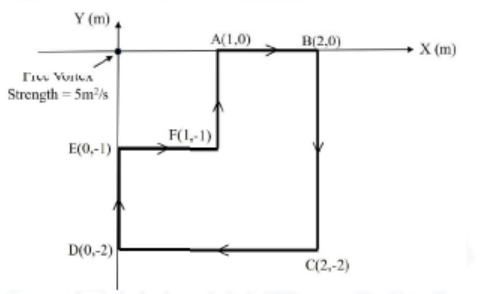
\includegraphics[width=0.5\columnwidth]{figs/im.png}
    \caption{}
    \label{fig:placeholder}
\end{figure}



\item 
A thin-walled cylindrical tank with closed ends, made of homogeneous and isotropic material, is pressurized internally. If the hoop (circumferential) strain developed in the material is thrice the value of the axial strain, then the Poisson's ratio of the material is \underline{\hspace{2cm}} \; \textit{(correct up to one decimal place).}

\hfill (GATE AE 2021)

\item 
A jet aircraft has the following specifications:
\begin{align*}
&\text{wing loading} = 1800~\text{N/m}^2, \quad \text{wing area} = 30~\text{m}^2,\\
&C_D = 0.02 + 0.04\,C_L^{\,2}, \quad C_{L,\max} = 1.6, \\
&\rho_{\text{sea level}} = 1.225~\text{kg/m}^3
\end{align*}
The speed at which the aircraft achieves maximum endurance in a steady and level flight at sea level is \underline{\hspace{2cm}}~\text{m/s} \; \text{(round off to two decimal places).}

\hfill (GATE AE 2021)
\item An aircraft with twin jet engines has the following specifications:  

Thrust produced (per engine) = 8000 N  

Spanwise distance between the two engines = 10 m  

Wing area = 50 m$^{2}$, Wing span = 10 m  

Rudder effectiveness, $C_{n\delta_{r}} = -0.002$/deg  

Density of air at sea level = 1.225 kg/m$^{3}$  

The rudder deflection, in degrees, required to maintain zero sideslip at 100 m/s in steady and level flight at sea level with a non-functional right engine is \underline{\hspace{2cm}} (round off to two decimal places).  

\hfill(GATE AE 2021)  

\item The velocity required to launch a space shuttle from the surface of the earth to achieve a circular orbit of 250 km altitude is \underline{\hspace{2cm}} (round off to two decimal places).  

For earth, $Gm_{e} = 398600.4 \;\text{km}^{3}/\text{s}^{2}$ and surface radius $R_{0} = 6378.14 \;\text{km}$.  

\hfill(GATE AE 2021)

\textbf{Q.26 -- Q.55 Multiple Choice Question (MCQ), carry TWO marks each (for each wrong answer: $-\dfrac{2}{3}$).}

\item A rigid massless rod pinned at one end has a mass $m$ attached to its other end. The rod is supported by a linear spring of stiffness $k$ as shown in the figure.  

\begin{figure}[H]
    \centering
    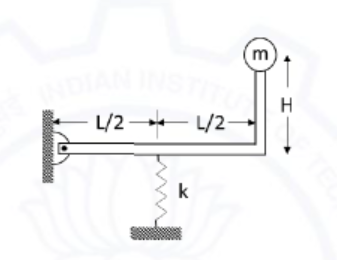
\includegraphics[width=0.5\columnwidth]{figs/image.png}
    \caption{}
    \label{fig:placeholder}
\end{figure}

The natural frequency of this system is \underline{\hfill}. \hfill (GATE AE 2021)

\begin{enumerate}
\begin{multicols}{2}
\item $\dfrac{1}{2\pi} \sqrt{\dfrac{kL^{2}}{4m(L^{2}+H^{2})}}$
\item $\dfrac{1}{2\pi} \sqrt{\dfrac{kL^{2}}{m(L^{2}+H^{2})}}$
\item $\dfrac{1}{2\pi} \sqrt{\dfrac{4kL^{2}}{m(L^{2}+H^{2})}}$
\item $\dfrac{1}{2\pi} \sqrt{\dfrac{k(L^{2}+H^{2})}{4mL^{2}}}$
\end{multicols}
\end{enumerate}
\item The figure shows three glasses P, Q and R with water and floating ice cube. Glass P has a solid ice cube, glass Q has an ice cube with a small solid steel ball embedded in it and glass R has an ice cube with an air bubble. After the ice cube melts, the level of water in glasses P, Q and R, respectively:

\hfill (GATE AE 2021)

\begin{figure}[H]
    \centering
    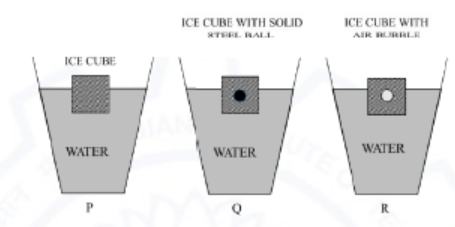
\includegraphics[width=0.5\columnwidth]{figs/image1.png}
    \caption{}
    \label{fig:placeholder}
\end{figure}

\begin{enumerate}
\begin{multicols}{2}
\item remains same, increases, and decreases  
\item increases, decreases, and increases  
\item remains same, decreases, and decreases  
\item remains same, decreases, and increases  
\end{multicols}
\end{enumerate}

\item To estimate aerodynamic loads on an aircraft flying at 100 km/h at standard sea-level conditions, a one-fifth scale model is tested in a variable-density wind tunnel ensuring similarity of inertial and viscous forces. The pressure used in the wind tunnel is 10 times the atmospheric pressure. Assuming ideal gas law to hold and the same temperature conditions in model and prototype, the velocity needed in the wind tunnel test-section is \underline{\hspace{2cm}}. \hfill (GATE AE 2021)

\begin{enumerate}
\begin{multicols}{2}
\item 25 km/h  
\item 50 km/h  
\item 100 km/h  
\item 20 km/h  
\end{multicols}
\end{enumerate}
\item The figure shows schematic of a set-up for visualization of non-uniform density field in the test section of a supersonic wind tunnel. This technique of visualization of high speed flows is known as:
\hfill (GATE AE 2021)
\begin{figure}[H]
    \centering
    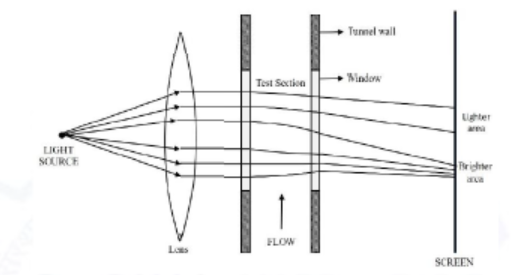
\includegraphics[width=0.5\columnwidth]{figs/fi1.png}
    \caption{}
    \label{fig:placeholder}
\end{figure}
\begin{enumerate}
\begin{multicols}{2}
\item schlieren  
\item interferometry  
\item shadowgraph  
\item holography  
\end{multicols}
\end{enumerate}



\item For a conventional fixed-wing aircraft in a 360$^{\circ}$ inverted vertical loop maneuver, what is the load factor ($n$) at the topmost point of the loop? Assume the flight to be steady at the topmost point.  

\hfill (GATE AE 2021)

\begin{enumerate}
\begin{multicols}{2}
\item $n = 1$  
\item $n < 1$  
\item $n = -1$  
\item $n > -1$  
\end{multicols}
\end{enumerate}



\textbf{ Q.31 - Q.36 Multiple Select Question (MSQ), carry TWO marks each (no negative marks).}

\item  
Which of the following statement(s) is/are true about the function defined as 
\[
f(x) = e^{x}|\cos x| \quad \text{for } x > 0 ?
\]
\hfill (GATE AE 2021)
\begin{enumerate}
\begin{multicols}{2}
\item Differentiable at $x = \tfrac{\pi}{2}$
\item Differentiable at $x = \pi$
\item Differentiable at $x = \tfrac{3\pi}{2}$
\item Continuous at $x = 2\pi$
\end{multicols}
\end{enumerate}



\item  
A two degree of freedom spring-mass system undergoing free vibration with generalized coordinates $x_1$ and $x_2$ has natural frequencies $\omega_1 = 233.9$ rad/s and $\omega_2 = 324.5$ rad/s, respectively. The corresponding mode shapes are 
\[
\phi_1 = \myvec{1 \\ -3.16}, 
\quad 
\phi_2 = \myvec{1 \\ 3.16}.
\] 
If the system is disturbed with certain deflections and zero initial velocities, then which of the following statement(s) is/are true?
\hfill (GATE AE 2021)
\begin{enumerate}
\item An initial deflection of $x_1(0) = 6.32 \, \text{cm}$ and $x_2(0) = -3.16 \, \text{cm}$ would make the system oscillate with only the second natural frequency.  

\item An initial deflection of $x_1(0) = 2 \, \text{cm}$ and $x_2(0) = -6.32 \, \text{cm}$ would make the system oscillate with only the first natural frequency.  

\item An initial deflection of $x_1(0) = 2 \, \text{cm}$ and $x_2(0) = -2 \, \text{cm}$ would make the system oscillate with a linear combination of first and second natural frequencies.  

\item An initial deflection of $x_1(0) = 1 \, \text{cm}$ and $x_2(0) = -3.16 \, \text{cm}$ would make the system oscillate with only the first natural frequency.  
\end{enumerate}

\item  
A shock moving into a stationary gas can be transformed to a stationary shock by a change in reference frame, as shown in the figure. Which of the following is/are true relating the flow properties in the two reference frames?

\hfill (GATE AE 2021)


\begin{figure}[H]
    \centering
    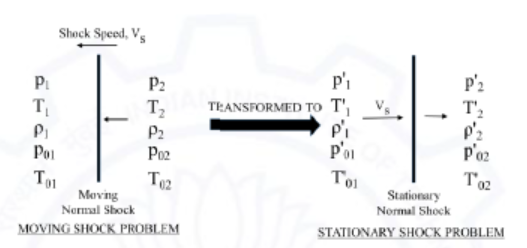
\includegraphics[width=0.5\columnwidth]{figs/dw.png}
    \caption{}
    \label{fig:placeholder}
\end{figure}

\begin{enumerate}
\begin{multicols}{2}
\item $T'_1 > T_1, \; T'_{01} > T_{01}, \; p'_{01} > p_{01}, \; \rho'_2 > \rho_1$
\item $T'_1 = T_1, \; T'_2 < T_{1}, \; p'_{01} > p_{01}, \; \rho'_2 = \rho_2$
\item $T'_1 < T_1, \; p'_1 > p_1, \; p'_{01} > p_{01}, \; \rho'_2 > \rho_1$
\item $T'_1 = T_1, \; p_2 > p_{01}, \; T'_{01} > T_{01}, \; p'_{01} > p_{01}$
\end{multicols}
\end{enumerate}

\item  
For a conventional fixed-wing aircraft, which of the following statements are true?

\hfill (GATE AE 2021)

\begin{enumerate}
\item Making $C_{m_\alpha}$ more negative leads to an increase in the frequency of its short-period mode.  

\item Making $C_{m_\alpha}$ more negative leads to a decreased damping of the short-period mode.  

\item The primary contribution towards $C_{l_p}$ is from the aircraft wing.  

\item Increasing the size of the vertical fin leads to a higher yaw damping.  

\end{enumerate}


\item  Which of the following statement(s) is/are true?

\hfill (GATE AE 2021)

\begin{enumerate}
\item Service ceiling is higher than absolute ceiling for a piston-propeller aircraft.

\item For a given aircraft, the stall speed increases with increase in altitude.

\item Everything else remaining the same, a tailwind increases the range of an aircraft.

\item For a jet aircraft constrained to fly at constant altitude, there exists an altitude where its range is maximum.
\end{enumerate}


\item  
A conventional fixed-wing aircraft, with a horizontal tail and vertical fin, in steady and level flight is subjected to small perturbations. Which of the following statement(s) is/are true?

\hfill (GATE AE 2021)


\begin{enumerate}
\item Vertical fin has a stabilizing effect on the lateral stability of the aircraft.

\item Vertical fin has a destabilizing effect on the directional stability of the aircraft.

\item Presence of wing anhedral increases the lateral stability of the aircraft.

\item Horizontal tail has a stabilizing effect on the longitudinal static stability of the aircraft.
\end{enumerate}

\item  
The ratio of the product of eigenvalues to the sum of the eigenvalues of the given matrix
\[
\myvec{3 & 1 & 2 \\ 2 & -3 & -1 \\ 1 & 2 & 1}
\]
is \underline{\hspace{2cm}} (round off to nearest integer).  
\hfill (GATE AE 2021)


\item  
The definite integral 
\begin{align*}
    \int_{1}^{5} x^3 \, dx
\end{align*}

is evaluated using four equal intervals by two methods - first by the trapezoidal rule and then by the Simpson's one-third rule. The absolute value of the difference between the two calculations is \underline{\hspace{2cm}} (round off to two decimal places).  
\hfill (GATE AE 2021)

\item  
The deflection \(y\) of a certain beam of length \(l\) and uniform weight per unit length \(w\), is given as  
\begin{align*}
    y = \frac{w}{48EI} \left( 2x^4 - 3lx^3 + l^3x \right),
\end{align*}

where \(x\) is the distance from the point of support and \(EI\) is a constant. The non-dimensional location \(\tfrac{x}{l}\), where the deflection of the beam is maximum, is \underline{\hspace{2cm}} (round off to two decimal places).  
\hfill (GATE AE 2021)

\item A large water tank is fixed on a cart with wheels and a vane (see figure). The wheels of the cart provide negligible resistance for rolling on the fixed support. The cart is tied to the fixed support with a thin horizontal rope. There is a hole of diameter $5\,\text{cm}$ on the side of the tank through which a jet of constant velocity of $10\,\text{m/s}$ emerges. The jet of water is deflected by the attached vane by $60\degree$ (see figure). Assume that the jet velocity remains constant at $10\,\text{m/s}$ after emerging from the vane. Take density of water to be $1000\,\text{kg/m}^{3}$. The tension in the connecting rope is \underline{\hspace{2cm}} N (round off to one decimal place).
\begin{figure}[H]
    \centering
    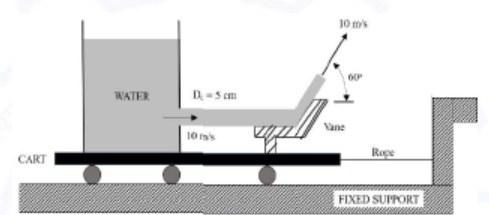
\includegraphics[width=0.5\columnwidth]{figs/fgfs.png}
    \caption{}
    \label{fig:placeholder}
\end{figure}
\hfill (GATE AE 2021)

\item 
A finite wing of elliptic planform with aspect ratio $10$, whose section is a symmetric airfoil, is placed in a uniform flow at $5\degree$ angle of attack. The induced drag coefficient for the wing is  \underline{\hspace{2cm}} (round off to three decimal places).
\hfill (GATE AE 2021)
\item 
Consider a model of a boundary layer with the following velocity profile:  

\[
\frac{u}{U} = 
\begin{cases} 
\left( \dfrac{y}{\delta} \right)^2 & y \leq \delta \\[6pt]
1 & y > \delta
\end{cases}
\]

The shape factor, defined as the ratio of the displacement thickness to momentum thickness, for this profile is \underline{\hfill} (round off to 2 decimal places).  
\hfill (GATE AE 2021)

\item 
An aircraft with a turbojet engine is flying at $270$ m/s. The enthalpy of the incoming air at the intake is $260$ kJ/kg and the enthalpy of the exhaust gases at the nozzle exit is $912$ kJ/kg. The ratio of mass flow rates of fuel and air is equal to $0.019$. The chemical energy (heating value) of fuel is $44.5$ MJ/kg and the combustion process is ideal. The total loss of heat from the engine to the ambient is $25$ kJ per kg of air. The velocity of the exhaust jet is \underline{\hfill} m/s (round off to two decimal places).  
\hfill (GATE AE 2021)

\item 
Hot gases are generated at a temperature of $2100$ K and a pressure of $14$ MPa in a rocket chamber. The hot gases are expanded ideally to the ambient pressure of $0.1$ MPa in a convergent-divergent nozzle having a throat area of $0.1 \,\text{m}^2$. The molecular mass of the gas is $12 \,\text{kg/kmol}$. The ratio of specific heats $(\gamma)$ of the gas is $1.32$. The value of the universal gas constant $(R_0)$ is $8314 \,\text{J/kmol-K}$. The acceleration due to gravity, $g$, is $9.8 \,\text{m/s}^2$. The specific impulse of the rocket is \underline{\hfill} seconds (round off to two decimal places).  
\hfill (GATE AE 2021)

\item 
A twin-spool turbofan engine is operated at sea level $(p_a = 1~bar,\; T_a = 288~K)$. The engine has separate cold and hot nozzles. During static thrust test at sea level, the overall mass flow rate of air through the engine and the cold exhaust temperature are measured to be $100~kg/s$ and $288~K$, respectively. The parameters for the engine are: \\
Fan pressure ratio $= 1.6$ \\
Overall pressure ratio $= 20$ \\
Bypass ratio $= 3.0$ \\
Turbine entry temperature $= 1800~K$ \\
The specific heat at constant pressure $(C_p)$ is $1.005~kJ/kg-K$ and the ratio of specific heats $(\gamma)$ is $1.4$ for air. \\
Assuming ideal fan and ideal expansion in the nozzle, the sea-level static thrust from the cold nozzle is \underline{\hspace{2cm}} kN (round off to two decimal places).  

\hfill (GATE AE 2021)

\item 
At the design conditions, the velocity triangle at the mean radius of a single stage axial compressor is such that the blade angle at the rotor exit is equal to $30\degree$. The absolute velocities at the rotor inlet and exit are equal to $140~m/s$ and $240~m/s$, respectively. The flow velocities relative to the rotor at inlet and exit of the rotor are equal to $240~m/s$ and $140~m/s$, respectively.  
\begin{figure}[H]
    \centering
    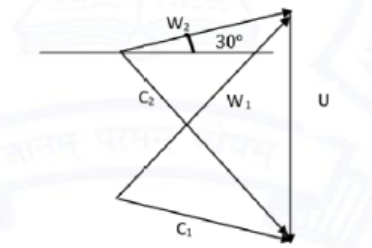
\includegraphics[width=0.5\columnwidth]{figs/46.png}
    \caption{}
    \label{fig:placeholder}
\end{figure}
The blade speed $(U)$ at the mean radius of the rotor is \underline{\hspace{2cm}} m/s (round off to two decimal places).  

\hfill (GATE AE 2021)

\item 
A single stage axial turbine has a mean blade speed of $340~m/s$ at design condition with blade angles at inlet and exit of the rotor being $21\degree$ and $55\degree$, respectively. The degree of reaction at the mean radius of the rotor is equal to $0.4$. The annulus area at the rotor inlet is $0.08~m^{2}$ and the density of gas at the rotor inlet is $0.9~kg/m^{3}$. The flow rate through the turbine at these conditions is \underline{\hspace{2cm}} kg/s (round off to two decimal places).  

\hfill (GATE AE 2021)

\item 
The air flow rate through the gas generator of a turboprop engine is $100~kg/s$. The stagnation temperatures at inlet and exit of the combustor are $600~K$ and $1200~K$, respectively. The burner efficiency is $90\%$ and the heating value of the fuel is $40~MJ/kg$. The specific heats at constant pressure $(C_p)$ for air and burned gases are $1000~J/kg-K$ and $1200~J/kg-K$, respectively. The flow rate of the fuel being used is \underline{\hspace{2cm}} kg/s (round off to two decimal places).  

(Note: Do not neglect the fuel flow rate with respect to the air flow rate)  

\hfill (GATE AE 2021)

\item 
A rigid horizontal bar ABC, with roller support at A, is pinned to the columns BD and CE at points B and C, respectively as shown in figure. The other end of the column BD is fixed at D, whereas the column CE is pinned at E. A vertical load $P$ is applied on the bar at a distance $a$ from point B. The two columns are made of steel with elastic modulus $200$ GPa and have a cross section of $1.5$ cm $\times$ $1.5$ cm. The value of $a$ for which both columns buckle simultaneously, is \underline{\hfill} cm (round off to one decimal place).
\hfill (GATE AE 2021)

\begin{figure}[H]
    \centering
    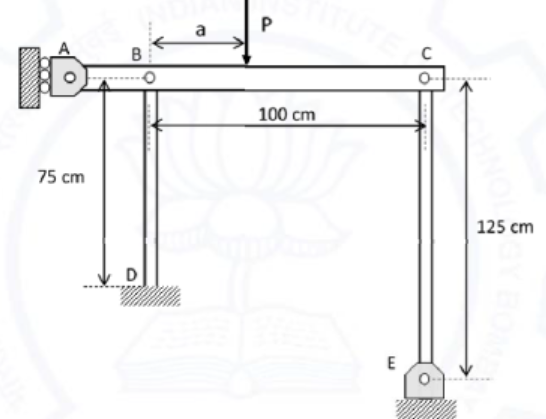
\includegraphics[width=0.5\columnwidth]{figs/49.png}
    \caption{}
    \label{fig:placeholder}
\end{figure}

\item 
A two-cell wing box is shown in the figure. The cell walls are $1.5$ mm thick and the shear modulus $G = 27$ GPa. If the structure is subjected to a torque of $12$ kNm, then the wall AD will experience a shear stress of magnitude \underline{\hfill} MPa (round off to one decimal place).
\begin{figure}[H]
    \centering
    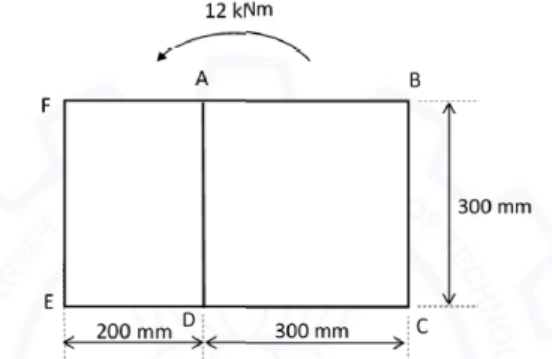
\includegraphics[width=0.5\columnwidth]{figs/50.png}
    \caption{}
    \label{fig:placeholder}
\end{figure}
\hfill (GATE AE 2021)

\item 
Two cantilever beams AB and DC are in contact with each other at their free ends through a roller as shown in the figure. Both beams have a square cross section of $50$ mm $\times$ $50$ mm, and the elastic modulus $E = 70$ GPa. If beam AB is subjected to a uniformly distributed load of $20$ kN/m, then the compressive force experienced by the roller is \underline{\hfill} kN (round off to one decimal place).
\begin{figure}[H]
    \centering
    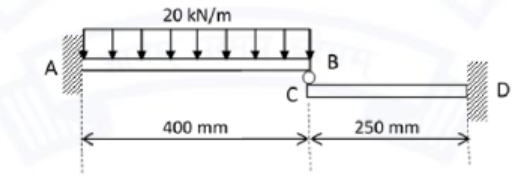
\includegraphics[width=0.5\columnwidth]{figs/51.png}
    \caption{}
    \label{fig:placeholder}
\end{figure}
\hfill (GATE AE 2021)

\item 
A $3~m \times 1~m$ signboard is supported by a vertical hollow pole that is fixed to the ground. The pole has a square cross section with outer dimension $250~mm$. The yield strength of the pole material is $240~MPa$. To sustain a wind pressure of $7.5~kPa$, the dimension $d$ of the pole is \underline{\hfill} mm (round off to nearest integer). \\
(Neglect the effect of transverse shear and load due to wind pressure acting on the pole)
\begin{figure}[H]
    \centering
    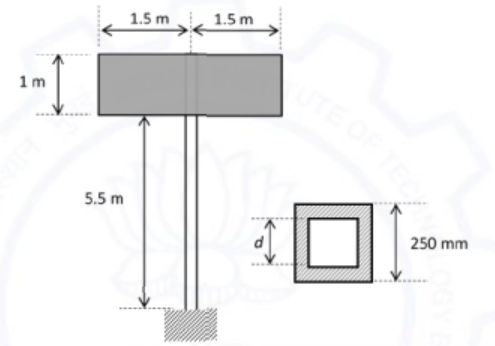
\includegraphics[width=0.5\columnwidth]{figs/52.png}
    \caption{}
    \label{fig:placeholder}
\end{figure}

\hfill (GATE AE 2021)

\item 
An airplane weighing $5500~kg$ is in a steady level flight with a speed of $225~m/s$. The pilot initiates a steady pull-up maneuver with a radius of curvature of $775~m$. The location of center of gravity (CG), center of pressure on wing (CP) and point of action (T) of tail force are marked in the figure. Use $g=9.81~m/s^{2}$. Neglect drag on the tail and assume that tail force is vertical. Assuming the engine thrust and drag to be equal, opposite and collinear, the tail force is \underline{\hfill} kN (round off to one decimal place).
\begin{figure}[H]
    \centering
    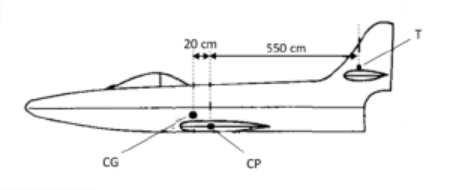
\includegraphics[width=0.5\columnwidth]{figs/53.png}
    \caption{}
    \label{fig:placeholder}
\end{figure}
\hfill (GATE AE 2021)

\item 
A jet aircraft weighing $10000~kg$ has an elliptic wing with a span of $10~m$ and area $30~m^{2}$. The $C_{D0}$ for the aircraft is $0.025$. The maximum speed of the aircraft in steady and level flight at sea level is $100~m/s$. The density of air at sea level is $1.225~kg/m^{3}$, and take $g=10~m/s^{2}$. The maximum thrust developed by the engine at sea level is \underline{\hfill} N (round off to two decimal places).

\hfill (GATE AE 2021)

\item 
Consider a jet transport airplane with the following specifications:

Lift curve slope for wing-body $\dfrac{\partial C_{L_{wb}}}{\partial \alpha_{wb}} = 0.1 \,/deg$

Lift curve slope for tail $\dfrac{\partial C_{L_t}}{\partial \alpha_t} = 0.068 \,/deg$

Tail area $S_t = 80~m^{2}$

Wing area $S = 350~m^{2}$

Distance between mean aerodynamic centers of tail and wing-body $\bar{l}_t = 28~m$

Mean aerodynamic chord $\bar{c} = 9~m$

Downwash $\varepsilon = 0.4\,\alpha$

Axial location of the wing-body mean aerodynamic center $x_{ac}/\bar{c} = 0.25$

Axial location of the center of gravity $x_{cg}/\bar{c} = 0.3$

All axial locations are with respect to the leading edge of the root chord and along the body $x$-axis. Ignore propulsive effects.

The pitching-moment-coefficient curve slope $(C_{m_\alpha})$ is \underline{\hfill} \,/deg (round off to three decimal places).

\hfill (GATE AE 2021)
\begin{center}
    \large\textbf{END OF THE QUESTION PAPER}
\end{center}

\end{enumerate}
\end{flushleft}
\end{document}